% \Main
% \hspace{0pt}
% \vfill
% \begin{center}
% ТЕОРЕТИЧЕСКАЯ ЧАСТЬ
% \end{center}
% \vfill
% \hspace{0pt}
% \pagebreak

\chapter{\centering\normalfont{ТЕОРЕТИЧЕСКАЯ ЧАСТЬ}}
\label{cha:ch_1}

\section{Постановка задачи}
В рамках данной выпускной квалификационной работы предполагается выбрать
компоненты для реализации и разработать инфраструктуру по поиску алгоритмов.

Инфраструктуру в целом требуется разработать в соответствии концепции
микросервисной архитектуры. Плюсом такой реализации является легкая заменяемость
модулей. Также необходимо средство контейнеризации и оркестрации контейнеров,
для более легкого развертывания приложений на облачных структурах
(вычислительных серверах).

Логика инфраструктуры будет заключаться в следующем:
\begin{itemize}
    \item Считать запрос пользователя. Т.е. предложить ему выбор вписать желаемое самому или выбрать из списка доступных опций;
    \item Произвести поиск по ключевым словам на необходимых интернет ресурсах;
    \item Выделить из возвращенных html страниц необходимые данные (произвести уточняющие запросы, либо запросы перехода на следующую страницу пагинации, если требуется);
    \item Полученные данные положить в базу данных;
    \item Пользователь теперь имеет возможность посмотреть, что нашлось.
\end{itemize}

\section{Микросервисная архитектура}
Для разработки приложения для данной выпускной квалификационной работы была выбрана микросервисная архитектура.
% https://ru.wikipedia.org/wiki/%D0%9C%D0%B8%D0%BA%D1%80%D0%BE%D1%81%D0%B5%D1%80%D0%B2%D0%B8%D1%81%D0%BD%D0%B0%D1%8F_%D0%B0%D1%80%D1%85%D0%B8%D1%82%D0%B5%D0%BA%D1%82%D1%83%D1%80%D0%B0
Микросервисная архитектура - такой вариант сервис-ориентированной архитектуры
программного обеспечения, который направлен на взаимодействие наиболее
раздробленных, небольших, слабосвязанных и легко модифицируемых модулей, которые
называются микросервисами.

У данной архитектуры есть ряд преимуществ и недостатков. Начнем с преимуществ:
\begin{itemize}
    \item модули (из которых состоит инфраструктура) легко заменяемые (не нужно
        полностью пересобирать и развертывать всю инфраструктуру, при внесении
        небольших изменений);
    \item сервисы могут быть реализованны с помощью разных средств, где
        последние выбираются в пользу высокой эффективности;
    \item архитектура получается симметричная, а не иерархическая.
\end{itemize}

Нельзя обойтись и без недостатков:
\begin{itemize}
    \item Сложность начальной разработки;
    \item Могут возникать сетевые издержки;
    \item Формат сообщений между сервисами должен быть стандартизован, что
        приводит к дополнительным издержкам на поддержание инфраструктуры.
\end{itemize}

Микросервисная архитектура также хорошо отвечает принципу единственной
обязанности -- Single Rsponsibility Principle\cite{microserv}, которое гласит:
«Собирайте вместе все, что изменяется по одной и той же причине и разделяйте
все, что изменяется по разным причинам».

% https://mcs.mail.ru/blog/prostym-jazykom-o-mikroservisnoj-arhitekture
Для сравнения, в монолитной архитектуре все компоненты соеденены в единое целое.
Вся логика по обработке запросов помещается внутрь одного процесса. Разумеется,
монолиты могут иметь модульную стркутуру -- содержать отдельные классы, функции.
Но связи между этими модулями настолько сильны, что изменение каждого из них
неизбежно отражается на работе приложения в целом. Визуальную демонстрацию
разницы между этими двумя архитектурами отображает рисунок \ref{fig:mon-vs-micr}.
\begin{figure}[H]
    \centering
    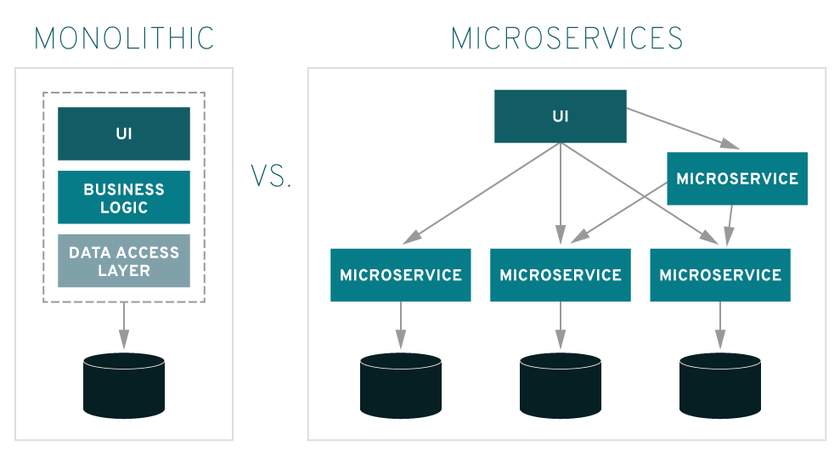
\includegraphics[scale=0.55]{inc/img/Monolithic-vs-microservices.png}
    \caption{Сравнение микросервисной и монолитной архитектуры}
    \label{fig:mon-vs-micr}
\end{figure}

\section{Технология контейнеризации}
% https://ru.wikipedia.org/wiki/%D0%92%D0%B8%D1%80%D1%82%D1%83%D0%B0%D0%BB%D0%B8%D0%B7%D0%B0%D1%86%D0%B8%D1%8F
По определению виртуализация -- это предоставление набора вычислительных
ресурсов или их логического объединения, абстрагированное от аппаратной
реализации, и обеспечивающее при этом логическую изоляцию друг от друга
вычислительных процессов, выполняемых на одном физическом ресурсе.

% https://habr.com/ru/company/southbridge/blog/530226/
% https://eternalhost.net/blog/razrabotka/docker-kubernetes
Одной из отличительных черт контейнеров от виртуальных машин -- то, что первые
используют возможность не железа, а операционной системы\cite{learning-docker},
так называемое пространство имен. Сравнение виртуальных машин и контейнеров
представленно в таблице \ref{tab:virt-cont}.
\begin{table}[H]
    \centering
    \caption{Сравнение виртуальных машин и контейнеров}
    \begin{tabular}{|l|l|}
        \hline
        Виртуальные машины & Контейнеры \\\hline
        Аппаратная виртуализация & Виртуализация на уровне ОС \\\hline
        Тяжеловесные             & Легковесные \\\hline
        Полностью изолированные  & Изолирование на уровне процессов \\
        (более безопасные)       & \\\hline
    \end{tabular}
    \label{tab:virt-cont}
\end{table}

Наглядная демонстрация архитектур виртуализации отображенно на рисунке
\ref{fig:virt-cont}.
\begin{figure}[H]
    \centering
    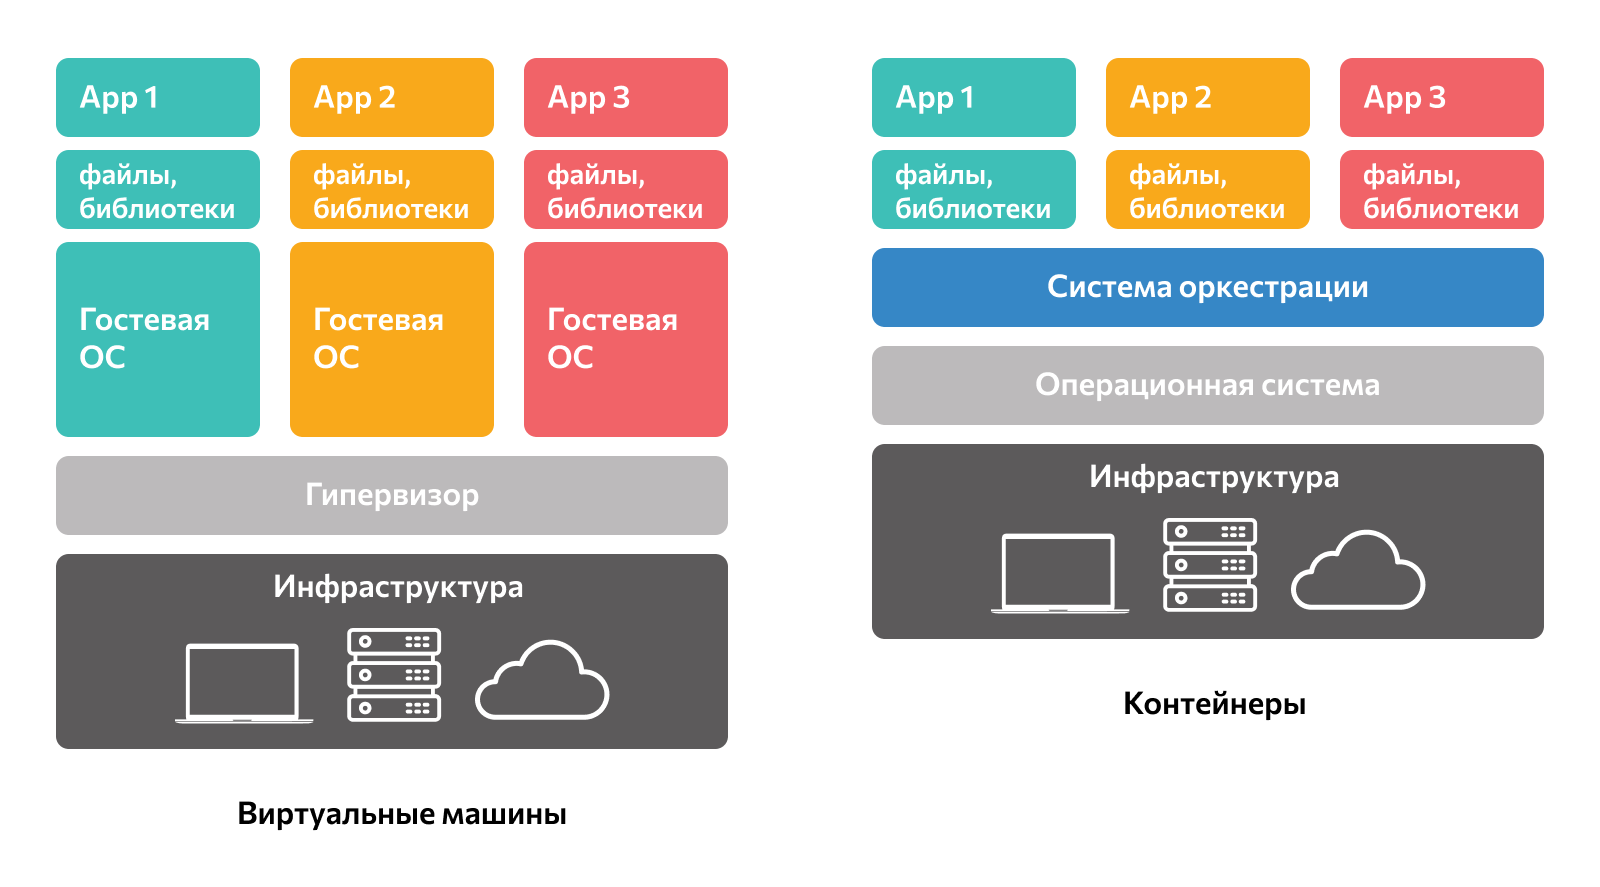
\includegraphics[scale=0.28]{inc/img/cont-vs-virt.png}
    \caption{Сравнение виртуальных машин и контейнеров}
    \label{fig:virt-cont}
\end{figure}

% https://blog.skillfactory.ru/glossary/kontejnerizacziya/
Технологии контейнеризации решают проблему изолированного запуска приложений и
рабочих сред вне зависимости от системы (должно быть то же ядро) и ПО,
установленных на конкретной машине. Также данная технология позволяет легко
управлять сложными приложениями и средами (упаковывать зависимости, перемещать
решение с системы на систему). 

% TODO: сравнение технологий контейнеризации
% TODO: рассказать про сами контейнеры и их структуру
% TODO: рассказать про отличие от картинок

\section{Поиск по web-ресурсам}
Для поиска по web-ресурсам безусловно достаточно только возможность совершать
HTTP-запросы (с необходимыми заголовками, сертификатами и т.д.) и читать то, что
сервер возвращает клиенту. Но в целях данной выпускной квалификационной работы
присутствует задача выбрать хорошую архитектуру. Поэтому нужно рассмотреть
фреймворки (или системы), которые позволяют упростить эту самую работу.

% https://pythobyte.com/10-tips-to-avoid-getting-blocked-while-scraping-websites-ncf-bee5b81c/
Также многие сайты стараются скрыть свою информацию от web-ботов. Возможно это
обусловленно тем, что последние злоупотребляют общедоступной информацией либо
вычислительной мощностью, которую сервер выделяет на пользователя. Поэтому, на
таких серверах могут быть настроенны политики запрета доступа к контенту при
слишком частом запросе страницы.

% https://coderlessons.com/tutorials/devops/uchitsia-scrapy/scrapy-kratkoe-rukovodstvo
Свойства которыми должен обладать фреймворк при работе с web-ресурсами:
\begin{itemize}
    \item Быть масштабируемым на большие проекты сканирования;
    \item Асинхронная обработка запросов;
    % TODO: сделать сноску на селекторы
    \item Встроенный механизм работы с селекторами;
    % TODO: сделать сноску на дросселирование
    \item Обладает механизмом автоматического дросселирования;
    \item Генерация результатов в разных структурных текстовых форматах.
\end{itemize}

% TODO: сравнение requests, beautiful soup 4, lxml, selenium, scrapy

Фреймворк на python -- scrapy удовлетворяет всем вышеперечисленным свойствам.
Более того для него написанна серверная часть scrapyd, которая позволяет
размещать пауков на мощных серверах, с последующим запуском либо по
расписанию, либо по http-запросу. Базовые компоненты scrapy и взаимодействия
между ними отображенны на рисунке \ref{fig:scrapy-arch}.
\begin{figure}[H]
    \centering
    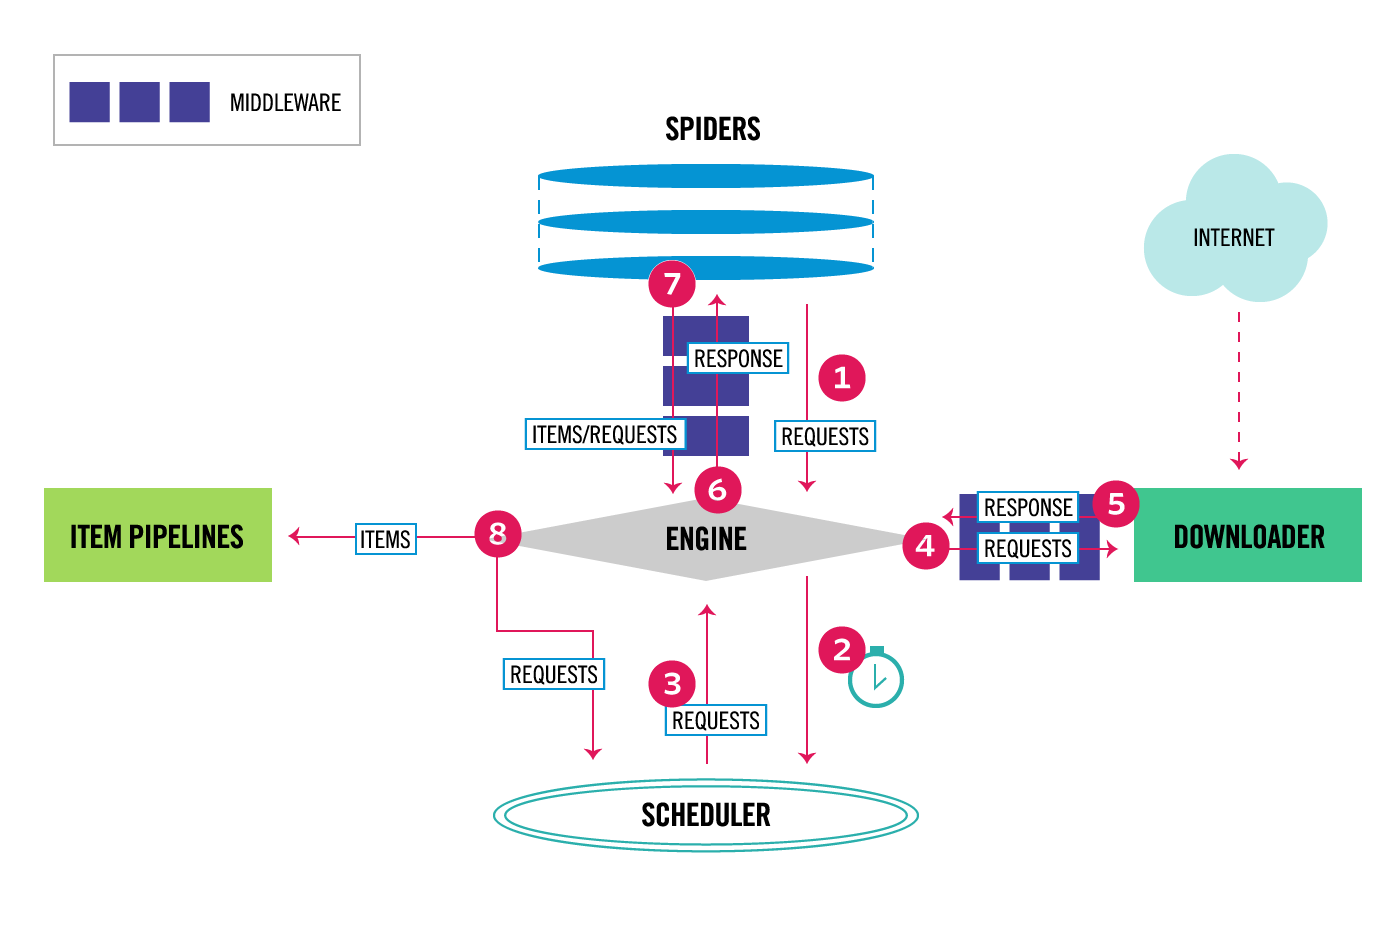
\includegraphics[scale=0.35]{inc/img/scrapy_architecture.png}
    \caption{Архитектура scrapy}
    \label{fig:scrapy-arch}
\end{figure}

% TODO: сделать сноску что этот файл обозначает
Также в этом модуле можно настроить много других политик доступа к интернет ресурсам. В такие политики входят:
\begin{itemize}
    \item Чтение файла \verb|robots.txt|;
    \item Лист прокси;
    \item Ротация заголвков и куков.
\end{itemize}

Данная библиотека позволяет полностью посмотреть список настроек, добавить свои,
и написать такую конфигурацию системы, чтобы не добавить свою вычислительную
сеть в черный список целевой структуры.

\section{Серверная часть}
\subsection{Web-сервер}
% https://ru.wikipedia.org/wiki/%D0%92%D0%B5%D0%B1-%D1%81%D0%B5%D1%80%D0%B2%D0%B5%D1%80
Веб-сервер -- сервер, принимающий HTTP-запросы от клиентов, обычно веб-браузеров,
и выдающий им HTTP-ответы, как правило, вместе с HTML-страницей, изображением,
файлом, медиа-потоком или другими данными. Веб-сервером называют как программное
обеспечение, выполняющее функции веб-сервера, так и непосредственно компьютер ,
на котором это программное обеспечение работает.

% https://developer.mozilla.org/ru/docs/Learn/Common_questions/What_is_a_web_server
На самом базовом уровне, когда браузеру нужен файл, размещённый на веб-сервере,
браузер запрашивает его через HTTP-протокол. Когда запрос достигает нужного
веб-сервера ("железо"), сервер HTTP (ПО) принимает запрос, находит запрашиваемый
документ (если нет, то сообщает об ошибке 404) и отправляет обратно, также через
HTTP. На рисунке \ref{fig:web-serv} показывается основопологающая функция
веб-сервера.
\begin{figure}[H]
    \centering
    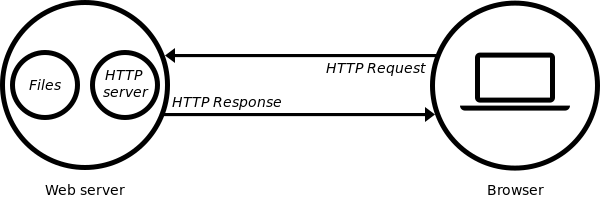
\includegraphics[scale=0.60]{inc/img/web-server.png}
    \caption{Принцип работы web-сервера}
    \label{fig:web-serv}
\end{figure}

Хранить ресурсы на выделенном web-сервере удобно по нескольким причинам:
\begin{itemize}
    \item Доступность выше чем у домашнего ПК;
    \item Всегда подключен к Интернету (зависит конечно же от хостера);
    \item Имеет статический IP адрес (с провайдерами обычно приходится договариваться на какую-то сумму, что бы выделили такой же);
    \item Обслуживается сторонней компанией, специализирующейся на предоставлении своего продукта.
\end{itemize}

% http://www.advanserv.ru/lab/stati/webserver/
% https://smoff.ru/howitworks/chto-takoe-nginx
Помимо своих основных функций веб-серверы выполняют и «работу» другого рода:
\begin{itemize}
    \item Запускает другие программные решения на серверных языках программирования;
    \item Защищает информацию от несанкционированного доступа;
    \item Ведет журнал обращений;
    % TODO: сделать сноску на два термина
    \item Обеспечивает аутентификацию и авторизацию;
    \item Обслуживает запросы разных типов: FTP, mailto и др.
\end{itemize}

% https://4db.github.io/2015/02/12/apache-iis-vs-nginx-nodejs/
На сегодняшний день популярными веб серверами являются: Apache, IIS, Nginx,
Node.js. У каждого веб сервера есть своя история, фокус на технологиях,
предпочитаемые ОС и многое другое. Но есть принципиальное различие в процессе
обработки запросов.

Apache, IIS используют обрабатывают каждый запрос в отдельном потоке/процессе -
“process-based”. Иллюстрация работы продемонстрированна на рисунке
\ref{fig:proc-based}.
\begin{figure}[H]
    \centering
    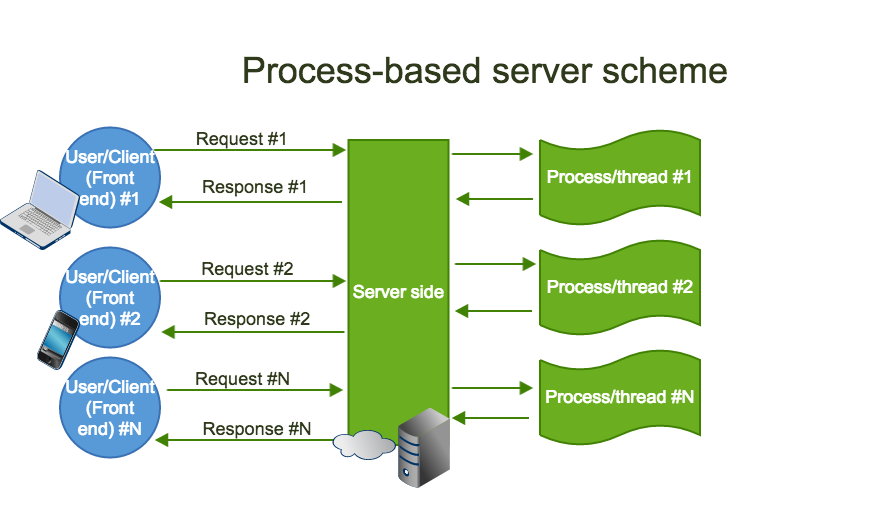
\includegraphics[scale=0.40]{inc/img/process-based-server.png}
    \caption{Схема работы Process-based веб серверов}
    \label{fig:proc-based}
\end{figure}

Event-based web serves: Nginx, Node.js. Работают на одном процессе/потоке,
используя все выделенные ресурсы. В единичном процессе/потоке(Singe
process/thread) используются все ресурсы веб сервера, позволяя обрабатывать
запросы максимально быстро, а в случаи задержки(получение данных от клиента,
отправки данных клиенту) работать с другими запросами из очереди(Event Queue)
т.е асинхронно. Иллюстрация работы продемонстрированна на рисунке
\ref{fig:event-based}.
\begin{figure}[H]
    \centering
    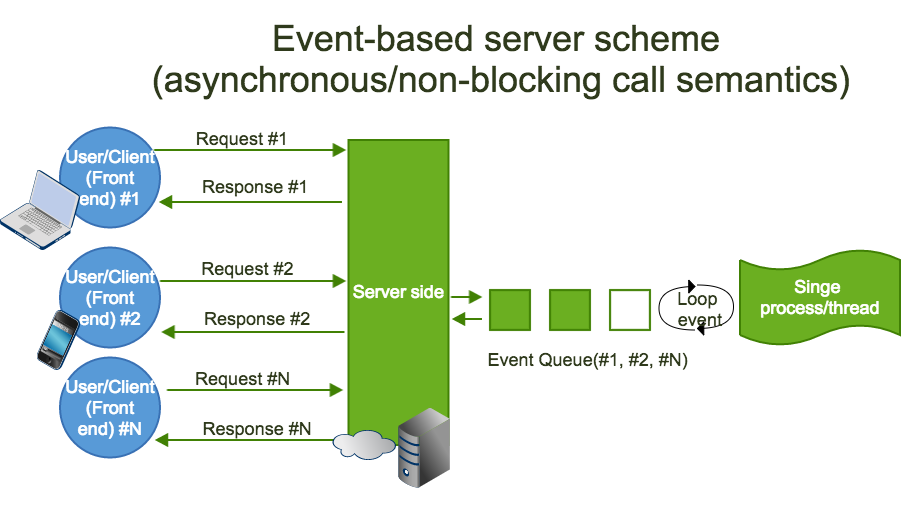
\includegraphics[scale=0.40]{inc/img/event-based-server.png}
    \caption{Схема работы Event-based веб сервера}
    \label{fig:event-based}
\end{figure}

Схема event-based(Node.js, Nginx) показывает большую производительность при
высоких нагрузках. Это связано с тем что не нужно делить ресурсы сервера между
другими потоками/процессами. Также серверные ресурсы всегда используются без
“простоя”.

Учитывая что Nginx обладает дополнительной функциональность (распределитель
нагрузки, вшитые механизмы защиты, прокси сервер), мой выбор пал именно на этот
web-сервер.

\subsection{Web-фреймворк}
% https://web-creator.ru/articles/about_frameworks
Фреймворки -- это программные продукты, которые упрощают создание и поддержку
технически сложных или нагруженных проектов. Фреймворк, как правило, содержит
только базовые программные модули, а все специфичные для проекта компоненты
реализуются разработчиком на их основе. Тем самым достигается не только высокая
скорость разработки, но и большая производительность и надёжность решений.

Веб-фреймворк -- это платформа для создания сайтов и веб-приложений, облегчающее
разработку и объединение разных компонентов большого программного проекта. За
счёт широких возможностей в реализациии бизнес-логики и высокой
производительности эта платформа особенно хорошо подходит для создания сложных
сайтов, бизнес-приложений и веб-сервисов.

Основное отличие библиотеки от фреймворка заключается в том, что последний не
просто дает разработчику нужный функционал, но еще и диктует правила построения
архитектуры приложения, задавая на начальном этапе разработки поведение по
умолчанию, формируя каркас, который нужно будет расширять и изменять согласно
указанным требованиям. Фреймворк также может включать вспомогательные программы,
библиотеки кода, язык сценариев и другое ПО, облегчающее разработку и
объединение разных компонентов большого программного проекта.

Для написания основной логики данной работы был выбран язык Python. Поэтому
рассмотрим основные web-фреймворки из которых стоит выбрать: Django и Flask.

% https://tproger.ru/articles/obzornyj-analiz-python-veb-frejmvorkov/
% TODO: Сделать сноску на MTV
Django диктует достаточно хорошую структуру (сразу подразумевает модульность и
расширяемость, модель MTV). Обширный каталог плагинов обеспечивают широкий выбор
опций для дополнения функциональности. Сразу при установке разработчику доступны
такие инсттрументы как ORM, шаблонизатор, мультиязычность, админ-панель,
автоматическая документация.

Flask позволяет разработчику собственноручно выбрать инструменты для реализации
логики. Обычно разработчики выбирают этот фреймворк для большего контроля над
проектом. По умолчанию Flask предоставляет:
\begin{itemize}
    \item Сервер разработки и отладчик;
    \item Интегрированные инструменты для модульного тестирования;
    \item Возможность отправки REST запросов;
    \item Шаблонизатор Jinja2;
    \item Пакеты-расширения, например flask-login, flask-sqlalchemy, flask-wtf.
\end{itemize}

Так как целевой проект должен получится сравнительно небольшим и по большей
части обучающим, то django слишком упростил бы разработку и не позволил бы
наглядно продемонстрировать используемые инструменты. Поэтому выбор пал на
flask.

\subsection{Коннектор}
% https://www.fullstackpython.com/wsgi-servers.html
% TODO: возможно просто описать стандарт wsgi и что это такое
Так как Nginx выступает в данной архитектуре как обратный прокси, необходим
способ запуска приложения для генерации динамического контента. UWSGI отвечает
за нагрузку приложения Flask с использованием интерфейса WSGI.

WSGI -- спецификация интерфейса. Он указывает какие методы следует использовать
для передачи запросов и ответов между сервером и приложением. Роль данного
интерфейса в общей архитектуре веб-сервера отображается на рисунке
\ref{fig:wsgi-web}.
\begin{figure}[H]
    \centering
    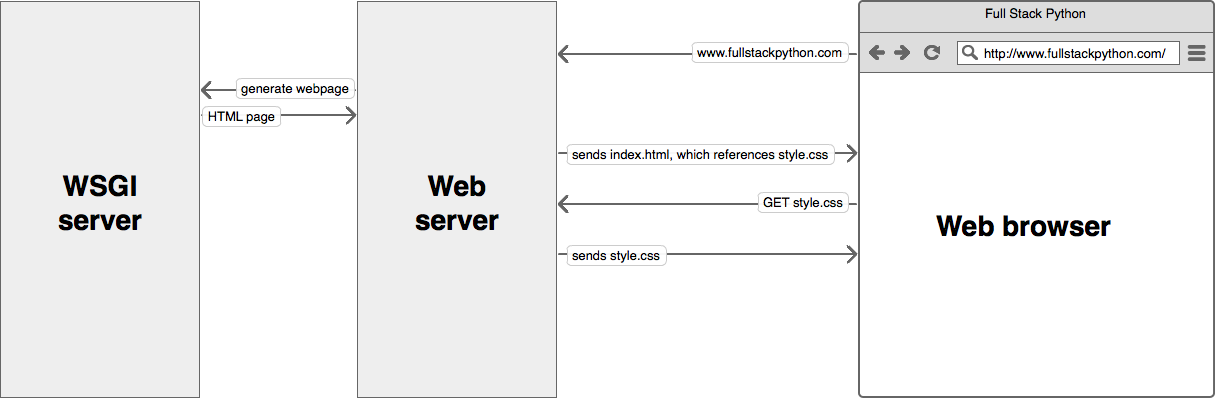
\includegraphics[scale=0.35]{inc/img/web-browser-server-wsgi.png}
    \caption{Роль WSGI сервера в архитектуре приложения}
    \label{fig:wsgi-web}
\end{figure}

\section{Брокер сообщений}
% https://ru.wikipedia.org/wiki/%D0%91%D1%80%D0%BE%D0%BA%D0%B5%D1%80_%D1%81%D0%BE%D0%BE%D0%B1%D1%89%D0%B5%D0%BD%D0%B8%D0%B9
Брокер сообщений -- архитектурный паттерн в распределённых системах; приложение,
которое преобразует сообщение по одному протоколу от приложения-источника в
сообщение протокола приложения-приёмника, тем самым выступая между ними
посредником. Кроме преобразования сообщений из одного формата в другой, в задачи
брокера сообщений также входит:
\begin{itemize}
    \item Проверка сообщений на ошибки;
    \item Маршрутизация конкретным приемникам;
    \item Разбиение сообщений на несколько маленьких, а затем агрегирование ответов приемников и отправка результата источнику;
    \item Сохранение сообщений в базе данных;
    \item Вызов веб-сервисов;
    \item Распространение сообщений подписчикам, если используются шаблоны типа издатель-подписчик;
\end{itemize}

Использование брокеров сообщений позволяет разгрузить веб-сервисы в
распределённой системе, так как при отправке сообщений им не нужно тратить время
на некоторые ресурсоёмкие операции типа маршрутизации и поиска приёмников. Кроме
того, брокер сообщений для повышения эффективности может реализовывать стратегии
упорядоченной рассылки и определение приоритетности, балансировать нагрузку и
прочее.

% https://habr.com/ru/post/466385/
Системы обмена сообщениями, как правило, предусматривают участие посредника
между двумя системами, которые взаимодействуют для дальнейшего расцепления
(разделения) отправителя от получателя или получателей. При этом система обмена
сообщениями позволяет отправителю отправить сообщение, не зная, где находится
получатель, активен ли он или сколько их экземпляров.

Первый паттерн обмена сообщениями -- Point-to-Point гарантирует что каждая
посылка будет доставлена хотя бы один раз. Классическая реализация такого
подхода производится через очереди, на которые подписываются один или несколько
потребителей. Каждое сообщениек доставляется только одному из подписанных
потребителей. Очереди обычнчо имеют свойство надежности -- они гарантируют, что
система обмена сообщениями будет хранить информацию до тех пор, пока потребитель
не подпишется на очередь для доставки сообщений. Иллюстрация данной архитектуры
отображается на рисунке \ref{fig:ptp}.
\begin{figure}[H]
    \centering
    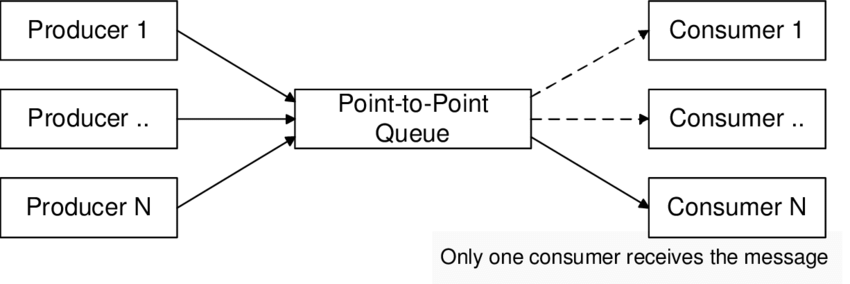
\includegraphics[scale=0.45]{inc/img/PTP-messaging-model.png}
    \caption{Модель обмена сообщениями Point-to-Point}
    \label{fig:ptp}
\end{figure}

Второй паттерн обмена сообщениями -- Publish-Subscribe гарантирует, что любой
подключившийся в настоящий момент получит сообщение. Классическая реализация
пподразумевает использование топиков. Когда сообщение отправляется в топик, оно
распределяется по всем подписанным пользователям. Топики ненадежные --
предоставляют гарантию доставки не более одного раза. Данный паттерн
используется, когда сообщения носят информационный характер, и потеря одного
сообщения -- не особо значима. Рисунок \ref{fig:pub-sub} отображает каким
образом работает данная модель обмена сообщениями.
\begin{figure}[H]
    \centering
    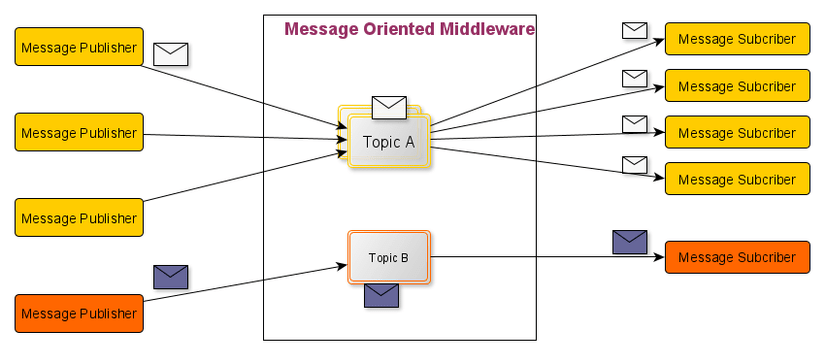
\includegraphics[scale=0.45]{inc/img/Publish-Subscribe-messaging-model.png}
    \caption{Модель обмена сообщениями Publish-Subscribe}
    \label{fig:pub-sub}
\end{figure}

% https://habr.com/ru/post/573358/
Выбрав несколько популярных брокеров сообщений, отобразим их характеристики и
запишем в таблицу \ref{tab:brok-comp}.
\begin{table}[H]
    \centering
    \caption{Сравнение брокеров сообщений}
    \begin{tabular}{|l|l|l|l|}
        \hline
        Broker                     & Kafka & RabbitMQ & SNS/SQS \\ \hline
        Локальный хостинг                & \checkmark  & \checkmark     &               \\ \hline
        Собственный хостинг              &             &                & \checkmark    \\ \hline
        Сторонний хостинг                & \checkmark  & \checkmark     &               \\ \hline
        Сложная маршрутизация            &             & \checkmark     & \checkmark    \\ \hline
        Высокая скорость передачи данных & \checkmark  &                &               \\ \hline
        Легкая установка                 &             &                & \checkmark    \\ \hline
    \end{tabular}
    \label{tab:brok-comp}
\end{table}

Для данной работы важны сохранность сообщений и возможность многократной
повторной обработки -- поэтому выбор пал на Kafka.

% TODO: вставить каким образом работает kafka

\section{СУБД}
% https://www.nic.ru/help/chto-takoe-subd_8580.html
Система управления базами данных (СУБД) -- это комплекс программно-языковых
средств, позволяющих создать базы данных и управлять данными. Иными словами,
СУБД -- это набор программ, позволяющий организовывать, контролировать и
администрировать базы данных.

% https://ru.wikipedia.org/wiki/%D0%A1%D0%B8%D1%81%D1%82%D0%B5%D0%BC%D0%B0_%D1%83%D0%BF%D1%80%D0%B0%D0%B2%D0%BB%D0%B5%D0%BD%D0%B8%D1%8F_%D0%B1%D0%B0%D0%B7%D0%B0%D0%BC%D0%B8_%D0%B4%D0%B0%D0%BD%D0%BD%D1%8B%D1%85
База данных -- совокупность данных, хранимых в соответствии со схемой данных,
манипулирование которыми выполняют в соответствии с правилами средств
моделирования данных. Для того, чтобы наглядно показать отличия СУБД от БД,
приведем рисунок \ref{fig:subd-bd-dif}.
\begin{figure}[H]
    \centering
    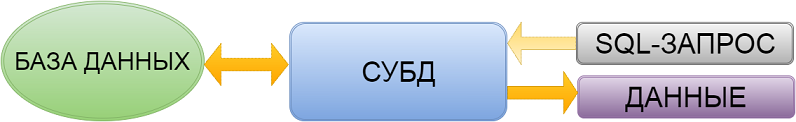
\includegraphics[scale=0.65]{inc/img/subd-bd.png}
    \caption{Чем отличаются СУБД и БД}
    \label{fig:subd-bd-dif}
\end{figure}

% https://www.parsec.ru/articles/obzor-sistem-upravleniya-bazami-dannykh-subd-dlya-sistem-kontrolya-i-upravleniya-dostupom-skud/
По способам доступа к базе данных делятся на следующие группы:
\begin{itemize}
    \item Клиент-серверные СУБД: обработка данных ведется в том же месте, где
        хранятся сами данные; к файлам данных имеет доступ только одна СУБД;
    \item Файл-серверные СУБД: приложения имеют доступ ко всем файлам базы
        данных; каждое приложение самостоятельно обрабатывает данные;
    \item Встраиваемые СУБД: поставляются в составе готового программного
        продукта; предназначены для локального хранения данных приложения и не
        рассчитаны на коллективное использование в сети;
\end{itemize}

Разница между файл-серверной СУБД и клиент-серверной СУБД отображена на рисунке
\ref{fig:file-client-serv-dif}.
\begin{figure}[H]
    \centering
    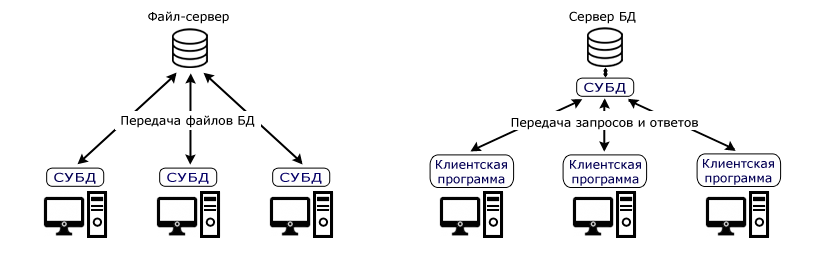
\includegraphics[scale=0.55]{inc/img/file-server-subd.png}
    \caption{Отличие файл-серверной СУБД от клиент-серверной СУБД}
    \label{fig:file-client-serv-dif}
\end{figure}

По модели данных СУБД делятся на следующие виды:
\begin{itemize}
    \item Иерархические;
    \item Сетевые;
    \item Реляционные;
    \item Объектно-ориентированные;
    \item Объектно-реляционные.
\end{itemize}

% https://ru.wikipedia.org/wiki/%D0%A1%D0%B8%D1%81%D1%82%D0%B5%D0%BC%D0%B0_%D1%83%D0%BF%D1%80%D0%B0%D0%B2%D0%BB%D0%B5%D0%BD%D0%B8%D1%8F_%D0%B1%D0%B0%D0%B7%D0%B0%D0%BC%D0%B8_%D0%B4%D0%B0%D0%BD%D0%BD%D1%8B%D1%85
Также СУБД бывают локальными (все части локальной СУБД размещаются на одном
компьютере) и распределенными (части СУБД могут размещаться не только на одном,
но на двух и более компьютерах).

% https://ru.wikipedia.org/wiki/NoSQL
NoSQL (от англ. not only SQL -- не только SQL) -- обозначение широкого класса
разнородных систем управления базами данных, существенно отличающихся от
традиционных реляционных СУБД с доступом к данным средствами языка SQL.
Применяется к системам, в которых делается попытка решить проблемы
масштабируемости и доступности за счёт полного или частичного отказа от
требований атомарности и согласованности данных.

Традиционные СУБД ориентируются на требования ACID к транзакционной системе:
атомарность (atomicity), согласованность (consistency), изолированность
(isolation), долговечность (durability), тогда как в NoSQL вместо ACID может
рассматриваться набор свойств BASE:
\begin{itemize}
    \item Базовая доступность (англ. basic availability) — каждый запрос гарантированно завершается (успешно или безуспешно);
    \item Гибкое состояние (англ. soft state) — состояние системы может изменяться со временем, даже без ввода новых данных, для достижения согласования данных;
    \item Согласованность в конечном счёте (англ. eventual consistency) — данные могут быть некоторое время рассогласованы, но приходят к согласованию через некоторое время.
\end{itemize}

% TODO: написать что-нибудь про теорему CAP

В зависимости от модели данных и подходов к распределённости и репликации в
NoSQL-движении выделяются четыре основных типа систем: «ключ — значение»
(key-value store), «семейство столбцов» (column-family store),
документоориентированные (document store), графовые. Основное отличие, а также
концепции NoSQL СУБД отображенны на рисунке \ref{fig:sql-vs-nosql}.
\begin{figure}[H]
    \centering
    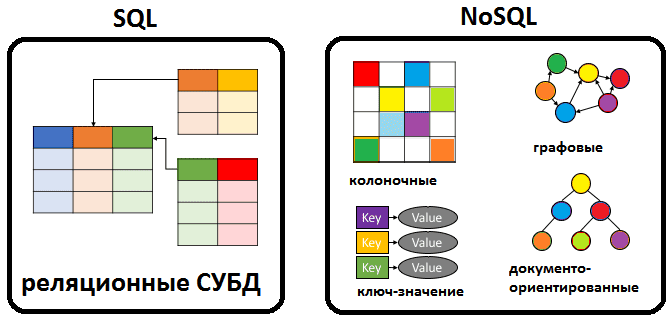
\includegraphics[scale=0.60]{inc/img/sql-vs-nosql.png}
    \caption{Сравнение SQL и NoSQL СУБД}
    \label{fig:sql-vs-nosql}
\end{figure}

% https://www.bigdataschool.ru/wiki/nosql
NoSQL СУБД обладает следующими преимуществами:
\begin{itemize}
    \item Линейная масштабируемость;
    \item Гибкость (использование полуструктурированных данных);
    \item Возможность работы с разными представлениями информации;
        % TODO: сделать сноску
    \item Высокая доступность за счет репликации данных и других механизом
        отказоустойчивости, в частности, шаринга (автоматического разделения
        данных по разным узлам сети);
    \item Производительность;
    \item Широкие функциональные возможности.
\end{itemize}

Обратной стороной преимуществ выступают:
\begin{itemize}
    \item Ограниченная емкость встроенного языка запросов;
    \item Сложности в поддержке всех ACID-требований к тразкациям (вследствии
        CAP модели);
    \item Сильная привязка приложения к конкретной СУБД.
\end{itemize}

Таким образом, для проектирования распределенной системы лучше всего подойдут
NoSQL СУБД. Так как работа предполагает текстовый поиск по базе данных, то выбор
пал на elastic search.

% TODO: написать подробнее о том, как работают различные NoSQL решения
% TODO: написать про фичи elastic search (можно задать маппинги, можно просто
% запушить документ)
% TODO: вставить инфу отсюда https://coderlessons.com/tutorials/bazy-dannykh/uchebnik-mongodb/2-uchebnik-po-nosql
% TODO: написать как работает elastic search
